\documentclass[../cheatSheetAlgoritmi.tex]{subfiles}
\begin{document}

\subsection{Esecitazione 2 - 29/10/19}
\textbf{Analisi - Ordinamento Funzioni}\\
Si consideri la seguente equazione di ricorrenza:
\begin{center}
	\begin{equation*}
  		T(n)=\begin{cases}
			T(m) +  T(n - m) & \text{$n > m$}\\
			1 & \text{$n \leq m$}	
  		\end{cases}
	\end{equation*}
\end{center}
dove \textit{m} è una costante intera positiva.\\
Si trovino, tramite il \textcolor{red}{metodo della sostituzione}, un limite superiore ed un limite inferiore per T(n). Fare particolare attenzione ai casi base.\\\\
\textbf{Soluzione}\\
Tentativo $T(n) = \mathcal{O}(n)$\\
$\exists c$ $>$ 0, $\exists m$ $\geq$ 0 : $T(n) \leq cn$, $\forall n$ $\geq$ $m$\\\\
\textbf{Ipotesi Induttiva}: $\forall k$ $>$ 0 $<$ n : T(k) $\leq$ ck\\
\textbf{Passo di Induzione}: Dimostriamo la disequazione per T(n)\\
$T(n) = T(m) + T(n-m) + 1 = 1 + cn - cm + 1 = cn - cm + 2 \stackrel{?}{\leq} cn \iff c \geq 2/m$\\
Poichè $m \geq 1$, $c \geq 2$ è un valore accettabile per ogni m.\\\\
\textbf{Caso Base}: Dimostriamo la disequazione per T(i) con $1 \leq i \leq m$\\
$T(i) = 1 \stackrel{?}{\leq} ci \iff c \geq 1/i$\\
Visto che $1 \leq i \leq m$ allora la disequazione è soddisfatta per $c \geq 1$.\\
Un valore di \textit{c} che soddisfa entrambe le disequazioni è ad esempio $c = 2$.\\\\
Abbiamo dimostrato il limite superiore, ora dobbiamo dimostrare il limite inferiore.\\
Tentativo $T(n) = \Omega(n)$\\
$\exists c$ $>$ 0, $\exists m$ $\geq$ 0 : $T(n) \geq cn$, $\forall n$ $\geq$ $m$\\\\
\textbf{Ipotesi Induttiva}: $\forall k$ $>$ 0 $<$ n : T(k) $\geq$ ck\\
$T(n) = T(m) + T(n-m) + 1 = 1 + cn - cm + 1 = cn - cm + 2 \stackrel{?}{\geq} cn \iff c \leq 2/m$\\
\textbf{Caso Base}: Dimostriamo la disequazione per T(i) con $1 \leq i \leq m$\\
$T(i) = 1 \stackrel{?}{\geq} ci \iff c \leq 1/i$\\
Il più piccolo valore trovato per le due disequazioni è $\frac{1}{m}$ dunque $c \leq 1/m$\\
Abbiamo dunque dimostrato che $T(n) = \Omega(n)$\\
Visto che abbiamo dimostrato i limiti superiori e inferiori $\implies$ $T(n) = \Theta(n)$\\\\
\textbf{SortinoSort}\\
Il professor Sortino ha inventato un nuovo algoritmo di ordinamento. Il vettore di input viene diviso in tre parti, di dimensioni approssimativamente uguali n/3. Dopo di che, vengono ordinati ricorsivamente le prime due parti del vettore (ovvero i primi due terzi), i secondi due terzi, e di nuovo i primi due terzi.
\begin{lstlisting}[ caption=SortinoSort]
SortinoSort(int[] A, int i, int j)
	if(j - i + 1) $\leq$ 6 then
		InsertionSort(A,i,j)
	else
		int s = ceil((j - i + 1)/3)
		SortinoSort(A, i, i + 2s - 1)
		SortinoSort(A, i + s, j)
		SortinoSort(A, i, i + 2s - 1)
\end{lstlisting}
\textbf{Soluzione}\\
L'equazione di ricorrenza del SortinoSort è del tipo seguente:
\begin{center}
	\begin{equation*}
  		T(n)=\begin{cases}
			3T(2n/3) & \text{$n > 6$}\\
			d & \text{$n \leq 6$}	
  		\end{cases}
	\end{equation*}
\end{center}
Dove d è il costo dell'InsertionSort visto che verrà usato quello per riordinare effettivamente il vettore passato in input e che ha una complessità nel caso medio/peggiore pari a $\mathcal{O}(n^{2})$.\\
A questo punto è possibile applicare il \textit{Master Theorem} per ricavare la forma chiusa dell'equazione di ricorrenza come segue: \\
$a = 3$, $b = \frac{3}{2}$, $\beta = 0$, , $\alpha = \log_b(a) = \log_\frac{3}{2}(3)$. \\
Possiamo osservare che $\alpha > \beta$, dunque vale che: $T(n) = \Theta(n^{\log_{\frac{3}{2}}(3)})$. \\ Questa complessità sarà sufficientemente bassa per finire sul libro del nostro amato Montresor? La risposta putroppo è no; il professor Sortino dovrà impegnarsi di più se vuole avere questo grande onore. Si può notare infatti che $\log_{\frac{3}{2}}(3)$ è un valore compreso tra 2 e 3 in quanto: $\frac{3}{2}^2 = \frac{9}{4} < 3$ $\frac{3}{2}^3 = \frac{27}{8} >3 $. \\ La ricorrenza ricavata è quindi $\Theta(n^2) < \Theta(n^{\log_{\frac{3}{2}}(3)}) < \Theta(n^3)$ che è peggiore di tutti gli algoritmi di ordinamento visti fino ad ora, fatta eccezione per il bogosort.\\\\
\newpage
\textbf{Alberi - Indovina l'albero}\\
Gli ordini di visita di un albero binario di 9 nodi sono i seguenti:

\begin{itemize}
	\item A, E, B, F, G, C, D, I, H (anticipato)
	\item B, G, C, F, E, H, I, D, A (posticipato)
	\item B, E, G, F, C, A, D, H, I (simmetrico).
\end{itemize}

Si ricostruisca l’albero binario e si illustri brevemente il ragionamento. \\\\
Per svolgere l'esercizio sono sufficienti le visite in ordine e le visite in preordine, in particolare grazie alla visita simmetrica siamo in grado di identificare i nodi che stanno nel sottoalbero di sinistra e quello di destra, mentre invece con la visita anticipata riusciamo non solo a determinare la radice ma anche i nodi che vegono visitati appena vengono raggiunti.\\
Infatti è possibile osservare che il nodo A è la radice dell'albero e nel suo sottoalbero sinistro vi sono: B, E, G, F, C, mentre in quello destro: D, H, I. \\
Il primo nodo alla sinistra di A è sicuramente E, come si osserva dalla visita anticipata. B è il figlio sinistro di E, mentre invece F è il suo figlio destro, e così via. \\É facile dunque ricostruire l'albero che segue: \\
\begin{center}
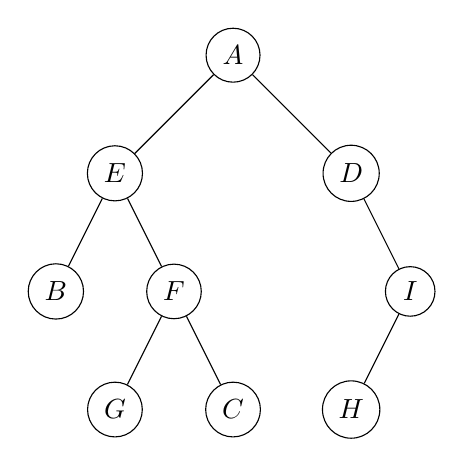
\begin{tikzpicture}[level distance=1.5cm,
	level 1/.style={sibling distance=3cm},
	level 2/.style={sibling distance=1.5cm}]
\node[circle,draw](z){$A$}
  child{
    node[circle,draw]{$E$} 
    	child{
    		node[circle,draw] {$B$}
    	} 
   	 	child{
   	 		node[circle,draw] {$F$}
   	 			child{
    				node[circle,draw] {$G$}
    			}
    			child{
    				node[circle,draw] {$C$}
    			} 
   	 	} 
   }
  child{
  	node[circle,draw]{$D$} 
  		child[missing]{
  		}
   	 	child{
   	 		node[circle,draw] {$I$}
   	 			child{
   	 				node[circle,draw] {$H$}
   	 			}
   	 			child[missing]{
   	 			}
   	 	} 
   };
\end{tikzpicture}
\end{center}

\textbf{Alberi – Albero livello–valore}\\
Scrivere un algoritmo che preso in input un albero binario T i cui nodisono associati ad un valore intero T.key, restituisca il numero di nodi dell’albero il cui valore è pari al livello del nodo. Vi ricordo che il livello del nodo è pari al numero di archi che devono essere attraversati per raggiungere il nodo dalla radice. Per cui la radice ha livello 0, i suoi figli hanno livello 1, etc.\\\\
La soluzione proposta è la seguente:
\begin{lstlisting}[ caption=Albero livello-valore]
int albero_livello_valore(TREE t)
	return dfs(T, 0)

int dfs(TREE T, int altezza)
	if T == nil then
   		return 0
  	else
		int costo = iif(T.key() == altezza, 1, 0)  	
  		return costo + dfs(T.right(), altezza + 1) + dfs(T.left(), altezza + 1)
\end{lstlisting}

Semplicemente è una dfs postordine, in cui viene sommato 1 se il valore chiave del nodo è pari al livello, mentre 0 altrimenti. Il livello viene aumentato di 1 mano a mano che ci si sposta dalla radice. \\\\
\textbf{Alberi – Albero livello–valore}\\
Dato un albero binario contenente interi, scrivere un algoritmo cherestituisca la lunghezza del più lungo cammino monotono crescente radice-discendente, dove:
\begin{itemize}
	\item il discendente non è necessariamente foglia;
	\item con lunghezza si intende il numero totale diarchi attraversati;
	\item con monotona crescente si intende che i valori contenuti nei nodidella sequenza devono essere ordinati in senso crescente da radice a discendente.
\end{itemize}

La soluzione proposta è la seguente:
\begin{lstlisting}[ caption=Percorso cammino-discendente]
int cammino(TREE t)
	return camminoRadiceDiscendente(t, nil, 0)

int camminoRadiceDiscendente(TREE t, int precedente, int lun)
  	if t == nil then
   		return lun
  	else
    	if precedente == nil or precedente $\geq$ t.value() then
      		return max(lun, camminoRadiceDiscendente(t.left, t.value, 0), camminoRadiceDiscendente(t.left, t.value, 0))
    	else
      		return max(camminoRadiceDiscendente(t.left, t.value, lun + 1), camminoRadiceDiscendente(t.left, t.value, lun + 1))
\end{lstlisting}

Questa soluzione prevede che sia tornata sempre la lunghezza massima del cammino incontrato fino ad ora avendo il riferimento al padre e facendo il controllo sul valore del figlio. Se il figlio è minore del padre allora la lunghezza del cammino corrente incrementa.
La soluzione di Montresor invece è molto più elegante:
\begin{lstlisting}[caption=Percorso cammino-discendente Montresor]
int monotone(TREE T)
	int maxl = 0
	int maxr = 0
	if T $\neq$ nil then
		if T.left() $\neq$ nil and T.left().value > T.value then
			maxl = 1 + monotone(T.left())
		if T.right() $\neq$ nil and T.right().value > T.value then
			maxr = 1 + monotone(T.right())
	return max(maxl, maxr)
\end{lstlisting}

\newpage
\end{document}